\section{Finite soft fields for arbitrary bounded tests}
\label{sec:buffers}

All measures in this section are nearest-neighbor Ising measures at
$K_c$.  In particular, a magnetic weight introduced here is an auxiliary
weight in a reference measure; it is not an interaction in the model of
\Cref{model:main}.  We write $\delta$ for the mesh after a buffer geometry
has been rescaled to fixed size.  A contour includes the lattice sites
needed for its nearest-neighbor Markov property.  Changes of this
convention by a bounded number of lattice layers will not affect any
positive clearance below.

The purpose of the section is to approximate the \emph{transmitted
effect} of a bounded observable.  The observable itself need not have a
scaling limit, nor need it be approximable pointwise by a function of
finitely many continuum fields.

\subsection{Reference charts and changes of continuation}

The reference geometries are the plane and a half-plane with homogeneous
fixed or free boundary.  In a half-plane chart we also allow lattice
domains whose physical boundaries, on successively larger windows,
converge to the line as single $C^1$ graphs.  The boundary prescription
is the same throughout the chart.  Such a chart admits reference
measures with the usual bulk spin convergence.  Indeed, first fix a
large window and continue its central boundary graph, by a cutoff, to
the limiting line outside a smaller window.  Close the resulting domain
with regular distant walls of the same boundary type.  The boundary
parametrizations and any marked arcs converge, so \Cref{in:fields}
applies.  The walls can subsequently be sent to infinity, or chosen to
increase sufficiently slowly with decreasing mesh.

For clarity, the lattice approximations needed in this construction
are compatible with site-induced domains.  A compact smooth boundary
has a finite cover by graph patches transverse to one of the coordinate
axes.  Within a smaller such patch, a nearby interior site can move in
the transverse coordinate into a region with positive interior
clearance; exterior sites have the corresponding property on their
side.  Lattice paths approximate paths in each buffered region.
This excludes alternating inside/outside diagonal pockets and gives
the requisite local connectivity and boundary convergence.  It also
allows regular inner charts to be chosen away from the ends of a
graph.  The finitely connected versions of \Cref{in:fields} will be used
when a pinned contour forms an inner boundary.

The dependence on a distant wall vanishes on fixed compact sets by
\Cref{in:patch}, iterated through annuli.  Thus these references give
the plane or half-plane spin formulas.  The same conclusion for
unbounded smeared tests follows from the moment bounds proved below.
All reference changes made before a fixed buffer limit have fixed
positive clearances.

We shall repeatedly use the following elementary consequence of the
pointwise ratio estimate.  It is useful to distinguish it from the
exceptional-probability assertion in \Cref{in:transfer}.

\begin{lemma}[Transport through an unchanged collar]
\label{buf:tilt}
Let $T$ be a separating contour and $W$ a farther contour, with a fixed
positive buffer between them.  Fix two outer Gibbs continuations,
independently of the data on the inner side of $T$.  They agree on the graph,
couplings, and fields between $T$ and $W$, and all their differences
are on or beyond $W$.  For any fixed data on the inner side of $T$,
the corresponding laws on $T$ differ by a positive tilt $w$ satisfying
\begin{equation}
 \frac{\sup w}{\inf w}\le K,
 \label{buf:tilt-bound}
\end{equation}
where $K$ depends only on the buffer geometry.  The same weight $w$
works for every change of the inner data.  Common pins and arbitrary
common finite fields are permitted wherever \Cref{in:ratio} permits
them.

If two laws $\nu_1,\nu_2$ on $T$ are compared in one continuation,
their laws in the other satisfy
\begin{equation}
 \norm{\nu_1^w-\nu_2^w}_{\TV}
 \le 2K\norm{\nu_1-\nu_2}_{\TV},
 \qquad
 d\nu_i^w=\frac{w\,d\nu_i}{\nu_i(w)}.
 \label{buf:tilt-tv}
\end{equation}
In the destination continuation, both tilted laws use the same further
Gibbs kernel given $T$.  Applying that kernel preserves the bound.
Remote data may first be conditioned on, or integrated out in the outer
Gibbs weights before the inner data are varied.
\end{lemma}

\begin{proof}
For a contour configuration $\tau$, let $Z_1^{\rm out}(\tau)$ and
$Z_2^{\rm out}(\tau)$ be the two outer continuation weights, including
any summation over remote data.  Their ratio
$w(\tau)=Z_2^{\rm out}(\tau)/Z_1^{\rm out}(\tau)$ is independent of
every inner datum.  For a fixed configuration
at $W$, \Cref{in:ratio} bounds the oscillation of this ratio over
$\tau$; normalization of the contour marginal does not change its
supremum-to-infimum ratio.  Conditioning at $W$ and mixing proves
\eqref{buf:tilt-bound} for an arbitrary continuation.  This argument
also applies to a different outer domain, since the graph in the
collar is unchanged.

Rescale $w$ so that $1\le w\le K$, and put
$d=\norm{\nu_1-\nu_2}_{\TV}$.  For an event $A$,
\[
 \left|\frac{\nu_1(w\one_A)}{\nu_1(w)}
       -\frac{\nu_2(w\one_A)}{\nu_2(w)}\right|
 \le Kd+|\nu_1(w)-\nu_2(w)|\le 2Kd.
\]
The bounds on the integrals follow from the layer-cake formula for
nonnegative functions bounded by $K$.  Taking the supremum over $A$
proves \eqref{buf:tilt-tv}.  Conditional on $T$, the actual outer Gibbs
kernel is the same for both inner laws, so applying that kernel cannot
increase total variation.
\end{proof}

Figure~\ref{fig:buffer} places this unchanged collar outside the
window reserved for a stopping barrier.  The contour $T$ carries the
common tilt for every barrier lying in that window.

\begin{figure}[!htbp]
\centering
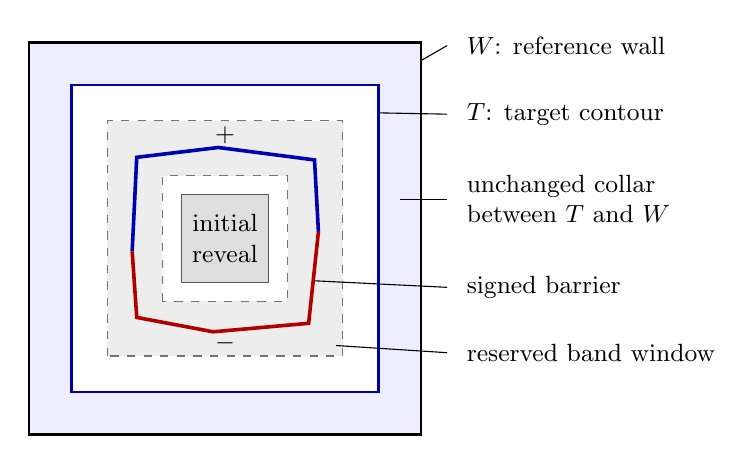
\begin{tikzpicture}[x=.83cm,y=.83cm,font=\small]
 \fill[blue!7] (-3,-3) rectangle (3,3);
 \fill[white] (-2.35,-2.35) rectangle (2.35,2.35);
 \fill[black!7] (-1.8,-1.8) rectangle (1.8,1.8);
 \fill[white] (-.96,-.96) rectangle (.96,.96);
 \draw[line width=.9pt] (-3,-3) rectangle (3,3);
 \draw[line width=.8pt,blue!65!black]
   (-2.35,-2.35) rectangle (2.35,2.35);
 \draw[dashed,black!55] (-1.8,-1.8) rectangle (1.8,1.8);
 \draw[dashed,black!55] (-.96,-.96) rectangle (.96,.96);
 \filldraw[fill=black!13,draw=black!65] (-.67,-.67) rectangle (.67,.67);
 \node[align=center] at (0,0) {initial\\reveal};
 \draw[line width=1.3pt,blue!70!black]
   (-1.42,-.2)--(-1.35,1.24)--(-.1,1.39)--(1.37,1.2)--(1.43,.1);
 \draw[line width=1.3pt,red!70!black]
   (1.43,.1)--(1.28,-1.3)--(-.18,-1.43)--(-1.35,-1.21)--(-1.42,-.2);
 \node at (0,1.58) {$+$};
 \node at (0,-1.6) {$-$};
 \node[anchor=west] at (3.55,2.95) {$W$: reference wall};
 \draw (3,2.72)--(3.4,2.95);
 \node[anchor=west] at (3.55,1.9) {$T$: target contour};
 \draw (2.35,1.92)--(3.4,1.9);
 \node[anchor=west,align=left] at (3.55,.6)
   {unchanged collar\\between $T$ and $W$};
 \draw (2.68,.6)--(3.4,.6);
 \node[anchor=west] at (3.55,-.75) {signed barrier};
 \draw (1.38,-.65)--(3.4,-.75);
 \node[anchor=west] at (3.55,-1.75) {reserved band window};
 \draw (1.7,-1.64)--(3.4,-1.75);
\end{tikzpicture}
\caption{One buffered source square, drawn schematically.  Dashed
squares delimit the reserved band window; the numerical stopping
levels are omitted.  The signed barrier separates the initial reveal
from $T$, with room for offsets and tip caps inside the window.
Changing the continuation beyond $W$ multiplies both laws on $T$ by
the same bounded-oscillation weight.}
\label{fig:buffer}
\end{figure}

\subsection{Deterministic barriers and soft fields}

For a bounded, piecewise regular profile $h$ with compact interior
support, set
\begin{equation}
 X_{\delta,h}=\delta^{15/8}\sum_{z}h(z)\sigma_z,
 \qquad
 U_{\delta,h}=
 \frac{\exp(X_{\delta,h})}{\E\exp(X_{\delta,h})}.
 \label{buf:weight}
\end{equation}
The expectation in the denominator is in the chosen homogeneous
reference law.  Profiles may be positive or negative.  Sampling their
fixed regular pieces on the lattice, with bounded lattice rounding of
their boundaries, is understood.

\begin{lemma}[Soft realization of a signed barrier]
\label{buf:barrier}
Fix a regular signed Jordan contour with finitely many sign arcs in an
interior square, a buffered outer target contour, and a more distant
square wall with a constant prescribed sign.  Given $\eta>0$, there is
a bounded piecewise regular
profile $h$, supported in arbitrarily small prescribed neighborhoods
of the signed contour, such that, for all sufficiently small $\delta$,
the law on the target with the contour pinned and the law tilted by
$U_{\delta,h}$ have total variation less than $\eta$.
The contour pins are not imposed in the latter law.  The profile and
all its nonzero tube widths are fixed before $\delta$ tends to zero.
The conclusion transfers through any unchanged outer buffer as in
\Cref{buf:tilt}, and can be applied successively to finitely many
disjoint buffered squares.
\end{lemma}

\begin{proof}
We compare the pinned law, the law with both pins and fields, and the
law with fields alone.  All error budgets in this proof may first be
divided by the finite transport constants in \Cref{buf:tilt}.

\paragraph{Fields in a pinned contour.}
Delete small neighborhoods of the finitely many sign switches.  Around
the remaining cores of the plus and minus arcs choose thin regular
tubes, with the matching field sign, and put zero field elsewhere.
The field has magnitude at least $h_0\delta^{15/8}$ on each tube core;
the finite number $h_0$ will be chosen last.  Fields on the inside of
the full pinned contour have no effect on its exterior.

Outside the contour, both the pinned law and the pinned-plus-field law
are between the following ordered laws.  For an upper law enlarge the
plus arcs into fully plus-pinned strips and omit the negative fields;
for a lower law use minus-pinned strips and omit the positive fields.
All original contour pins remain.  Strip shapes can be chosen as
regular bulges attached to just the corresponding sign arcs.  Their
ends stay away from the switches, and the outer wall is unchanged.
After integrating irrelevant components, the target components are
regular marked domains, possibly annular.  They converge back to the
original marked domain as the strip widths tend to zero.

Choose a square source contour $S_0$ beyond all strips and an
intermediate square cut $J$ between $S_0$ and the target, with fixed
pin-free collars.  At fixed positive strip widths,
\Cref{in:fields} gives convergence of the rescaled one-point functions
on $J$.  Their limits converge to those in the original domain when
the widths shrink.  They are uniformly bounded on $J$: its distance
from every pin is positive, and the fully wired one-arm bound controls
the absolute magnetization.  Consequently the difference of the
normalized magnetic sums on $J$ tends to zero.  In rescaled coordinates
this normalization is $\delta^{7/8}\sum_{z\in J}\sigma_z$, up to
fixed geometric factors.

For either of the two laws being compared, couple it in order below
the common upper law.  The magnetic difference is bounded by the full
upper-minus-lower difference.  The continuation from $S_0$ to the
target is identical in these comparisons, and has no field or changed
pin.  \Cref{in:ordered} therefore gives an arbitrarily small target-TV
distance.  This conclusion is uniform in $h_0$, because the extreme
pinned-strip laws do not depend on the field magnitude.

\paragraph{Pins in a soft field.}
Keep the positive tube widths just chosen.  Cover each arc core by
finitely many patches, each contained in the central third of a
square whose slightly larger buffered square is still inside the
matching-sign tube.  Consider first a plus patch and the comparison
law with free boundary on its larger square and homogeneous field
$h_0\delta^{15/8}$.

By the necklace input in \Cref{in:fields}, given $\xi>0$ there are
finite $K$ and $c>0$ such that, at sufficiently small mesh, with
probability at least $1-\xi$ the central square is surrounded by a
vertex circuit covered by at most $K$ critical FK clusters, each with
at least $c\delta^{-15/8}$ vertices.  Consecutive pieces may touch by
a nearest-neighbor step.  Equivalently, the event can be expressed
using connected subsets of that minimum size; it is then increasing
under addition of bonds.  The internal-bond law in the positive field
dominates the zero-field law.  Conditional on its internal clusters,
each qualifying cluster attaches to the plus ghost with probability
at least $\tanh(c h_0)$.  The usual conditional cluster formula, or
a union bound over the at most $K$ clusters, now gives a plus-spin
circuit with probability at least
\begin{equation}
 1-\xi-K\bigl(1-\tanh(c h_0)\bigr).
 \label{buf:necklace-plus}
\end{equation}
The same estimate holds for a larger matching positive field by
monotonicity.  Thus its failure probability can be made arbitrarily
small with a sufficiently large but finite $h_0$.

Across the buffer of the larger square, \Cref{in:ratio} compares this
local law to the actual one, uniformly in all common fields and
remote signs.  It multiplies the failure probability by a fixed
constant.  Matching pins inserted earlier inside the local chart
preserve the circuit event by monotonicity; other pins are covered by
the same comparison.  The argument for a minus patch is obtained by
spin flip.

Here is the coupling that turns the circuit estimate into a pinning
estimate.  Couple the law before a plus patch is pinned and the law
after it is pinned in stochastic order.  Start at the patch and
reveal, in order, the non-plus sites accessible from it by star
adjacency, together with their first plus boundary.  At each step
use the ordered conditional distributions of the next site.  This
is a finite adaptive spin reveal; conditional on its revealed spins,
the unobserved law is the original Gibbs continuation.  A
nearest-neighbor plus circuit in the lower configuration confines
the exploration before it reaches the target.  The separating plus
boundary is plus in both configurations.  The exterior conditional
laws are then identical and can be sampled together.  It follows
that the target-TV distance is at most the lower law's circuit
failure probability.  This uses a stopping reveal, rather than
conditioning on an arbitrarily selected random circuit.  For minus
pinning reverse the order.

Apply the construction to the finite patch cover, allocating the
variation budget among its members.  Pins still missing near sign
switches lie in finitely many small disks.  By \Cref{in:patch}, inserting
these pins changes the target law by an arbitrarily small amount,
uniformly in the fields and the other pins.  Thus the field-only law
and the pinned-plus-field law are close on the target.

The choices have the required order: first make the switch
neighborhoods small; next make the strips thin but of positive
width; next choose a sufficiently large finite $h_0$; finally choose
the mesh small enough.  The first comparison was uniform in $h_0$.
Combining the two comparisons proves the local statement.
\Cref{buf:tilt} transports each comparison to any allowed
continuation.  For finitely many disjoint squares, condition on all
other pins or fields and telescope; their differences remain beyond
the square's outer buffer.
\end{proof}

\subsection{Uniform replacement of bounded observables}

Fix concentric buffer geometries with inner scale $s$ and outer scale
$R$, where $R/s$ is a sufficiently large fixed number.  An inner
observable is supported in $B_s$, and an outer observable is supported
on or beyond $\partial B_{R/2}$.  There is room for a fixed-factor
buffer at either end.  In a half-plane chart the center is on the
limiting boundary line.  Constants denoted $c,C>0$ below depend only
on these fixed support and separation factors.  In particular, they
do not depend on an approximation tolerance.

\begin{lemma}[Finite soft-weight replacement]
\label{buf:soft}
In the preceding reference geometries, for every $\eta>0$ there is a
finite list of bounded piecewise regular profiles $h_1,\ldots,h_N$,
and a fine-mesh threshold, such that every inner observable $F_\delta$
with $\norm{F_\delta}_\infty\le1$ has coefficients
$c_1(\delta),\ldots,c_N(\delta)$ satisfying
\begin{equation}
 \sum_{i=1}^N|c_i(\delta)|\le1,
 \qquad
 \sup_{\norm{H_\delta}_\infty\le1}
 \left|\E[F_\delta H_\delta]
       -\sum_{i=1}^N c_i(\delta)
                    \E[U_{\delta,h_i}H_\delta]\right|<\eta.
 \label{buf:one-side}
\end{equation}
The supremum is over all outer observables, including the constant
one.  The profiles and threshold are independent of $F_\delta$ and
$H_\delta$.  The coefficients may depend on the mesh and on the
observable.  The analogous statement holds with the inner and outer
roles reversed.

Inner replacement profiles can be supported within distance $Cs$
of the center; outer replacement profiles can be supported where
$cR\le |z|\le CR$.  The two profile regions have a fixed relative
radial separation.  Each profile is supported in a compact interior
set avoiding the center, with additional positive clearances that
may depend on $\eta$.

More precisely, let $(F_{\alpha,\delta})_{\alpha=1}^p$ and
$(H_{\beta,\delta})_{\beta=1}^q$ be finite families of inner and outer
observables, all of sup norm at most one.  There are finite inner and
outer profile lists $(h_i)$ and $(g_j)$ and coefficient vectors
$c_{\alpha i}(\delta),d_{\beta j}(\delta)$ such that
\begin{gather}
 \sum_i|c_{\alpha i}(\delta)|\le1,\qquad
 \sum_j|d_{\beta j}(\delta)|\le1,\label{buf:matrix-mass}\\
 \left|\E[F_{\alpha,\delta}H_{\beta,\delta}]
 -\sum_{i,j}c_{\alpha i}(\delta)d_{\beta j}(\delta)
       \E[U_{\delta,h_i}U_{\delta,g_j}]\right|<\eta
 \quad\text{for every }\alpha,\beta.\label{buf:two-side}
\end{gather}
The same row and column vectors work throughout this matrix.  Adjoin
the zero profile, for which $U_{\delta,0}=1$, to each list.  A constant
observable can then be retained exactly; adjoining it to either family
controls all the separate means with the same coefficients.  The
profile lists and mesh threshold are independent
of the observables.  The preceding support bounds apply to both lists.
Parity and plane lattice-rotation symmetries may be imposed by averaging.
The same conclusions hold along the approaching-half-plane charts
described above.
\end{lemma}

\begin{proof}
We first prove the one-sided assertion.  Smooth the observable by
conditioning on a separating square contour at its end of the
buffer.  For the outer observable, a square just inside $B_{R/2}$
can be used.  The conditional mean is bounded by one, and replacing
the observable by that mean preserves its pairings with all tests on
the other side of the cut.

Break the contour at its corners and, in a boundary chart, at its
intersections with the physical boundary.  Choose intersections
transversely and away from corners, or include a coincident corner
in the same deletion.  Delete short pieces in small disks at these
points.  The values in a deleted piece can be assigned arbitrarily
in the far conditional law, at a cost tending to zero by
\Cref{in:patch}.  More explicitly, average the original bounded
contour function over the deleted spins conditional on the retained
ones.  For every assignment of the retained spins, compare the far
law for each deleted-spin assignment to a single prescribed one.
The uniform pointwise ratio bound controls the resulting pairing
error.  Comparing that prescribed law back to the conditional mixture
costs the same bound.  Thus the new pairing is again in the original
reference measure, with the conditionally averaged contour function.
This operation does not assert a pointwise approximation of
the observable.  It also handles the vanishing displacements of
intersection points in an approaching boundary chart.

The retained segments have positive distance from the physical edge
and from the far test.  Subdivide them into finitely many sufficiently
short straight pieces, and delete much smaller gaps at the subdivision
points by the same argument.  Each piece now lies strictly inside its
own square, and these squares have disjoint enlarged buffers.  The buffers may be thin: for adjacent pieces of length $\ell$ separated
by a gap $g$, one may take square half-sides just above $\ell/2$ and
outer walls at $\ell/2+g/4$, with strictly nested band and target levels
in between. The stopping theorem allows any such fixed positive
clearances \cite[Remark~7.1]{IsingToolkit}; its constants need not be uniform as $g/\ell$ shrinks.
Choose the piece lengths after the original corner and physical-edge
deletions, smaller than their positive geometric clearances. This also
keeps squares on different sides disjoint. All these sizes and their
number are fixed before the mesh limit.  The
observable, for the purpose of the desired pairings, has become a
bounded function of spins in these finitely many source squares.

In each square reveal an interior square containing its source piece
and apply the outward part of \Cref{in:transfer}.  Choose a separating
target square contour $T$ outside the stopping band, and a more
distant constant-sign reference wall $W$, both still inside the
square's buffer; see \Cref{fig:buffer}.  The theorem gives finitely
many deterministic regular signed barriers.  Off an exceptional
descriptor, adding the chosen barrier changes the reference target
law by the prescribed small total-variation amount, for every
realizable stopping transcript.

The actual continuation can include all other source squares, their
transcripts, and the physical boundary.  These data lie beyond $W$.
The law on $T$ is therefore tilted by the common weight in
\Cref{buf:tilt}, independently of the transcript and its replacement.
The per-transcript TV estimate transports to this continuation.
Its further law is the same given $T$.  The exceptional probability
is still small, by the buffered comparison for the band marginal.
Thus both required parts of the stopping theorem transport: the
exceptional-event estimate uses the band density, and the conditional
target estimate uses the common target-contour tilt.

Apply these comparisons successively to the finite family of source
squares.  Conditional on their transcripts the remaining law is
Gibbs with the revealed pins.  Each square's unchanged outer collar
permits the same conditional comparison, so the errors telescope.
After all barriers have been inserted, they separate the initially
observed spins from every far test.  The law for the latter is the
original reference law with just the selected deterministic signed
barriers imposed; it no longer depends on the transcript behind them.

Let $A_i$ be the good descriptor bins, with a joint index if several
squares are used.  The corresponding coefficient is
\[
 c_i(\delta)=\E[F_\delta\one_{A_i}],
 \qquad
 \sum_i|c_i(\delta)|
 \le\E[|F_\delta|\one_{\cup_i A_i}]\le1.
\]
Here $F_\delta$ denotes the bounded function after the initial
conditioning and deletions.  Its pairings already differ from the
original ones by only the allocated error.  Exceptional bins
contribute at most their probabilities.  We have therefore obtained
a signed combination of deterministic pinned laws with coefficient
mass at most one, uniformly against every bounded far test.

Apply \Cref{buf:barrier} to every member of the finite barrier list.
For a joint barrier choice, add the profiles in its disjoint squares.
The field-only measure is exactly the original reference measure
tilted by the single normalized weight for this sum profile.
Normalization is global; no product of local normalizing constants
is assumed.  The coefficient mass does not change.  Allocate the
remaining errors among the finitely many choices and squares.
This proves \eqref{buf:one-side}.

All source squares were placed on fixed-factor contours at the
observable's end of the original collar.  Consequently their
profiles remain within $Cs$ at the inner end, or between $cR$ and
$CR$ at the outer end, regardless of how small the deletion disks,
strip widths, or approximation tolerances are chosen.  They avoid
the center.  The deletion and subdivision choices put them strictly
in the interior, also in boundary charts.  This proves the support
claims.

If a finite symmetry group preserves the reference law and the
geometry, average the replacement over that group, with its
appropriate character for an odd observable.  Enlarge the finite
profile list by the corresponding images.  The sum of absolute
coefficients cannot increase.  In the plane this includes the
right-angle lattice rotations and spin flip; free boundary also
permits spin flip.

The two-sided finite-array assertion requires uniform integrability
when a soft weight replaces one of the original bounded tests.  We
give its proof after establishing the required moment bounds in
\Cref{buf:moments}.  The preceding one-sided construction is
independent of those bounds.
\end{proof}

\subsection{Moments and the order of the two replacements}

\begin{lemma}[Smeared moments and exponential tails]
\label{buf:moments}
Let $h_1,\ldots,h_m$ be fixed bounded piecewise regular profiles with
compact interior supports in a reference chart.  All joint polynomial
moments of the variables $X_{\delta,h_i}$ converge to the integrals
of the corresponding continuum spin correlations.  For every
$t<\infty$,
\begin{equation}
 \sup_{\delta\ \mathrm{small}}
 \E\exp\!\left(t\sum_{i=1}^m|X_{\delta,h_i}|\right)<\infty.
 \label{buf:exponential}
\end{equation}
Joint exponential expectations converge as well.  In particular the
weights in \eqref{buf:weight} have convergent normalizations and
uniformly integrable powers of every fixed positive order.

For two separated support regions with a fixed buffer, there is a
geometric constant $K$ such that
\begin{equation}
 \E[A U_{\delta,g}]\le K\E A
 \label{buf:weighted-tail}
\end{equation}
for every nonnegative function $A$ of the first region and every
normalized positive soft weight on the second.  The constant is
independent of $g$, its magnitude, and its complexity.
\end{lemma}

\begin{proof}
First consider one compact set.  Buffered comparisons reduce bounds
on nonnegative functions there to bounds in the plane, or to a fixed
homogeneous square reference.  The standard two-point estimate is
\[
 \delta^{-1/4}\bigl|\E[\sigma_z\sigma_{z'}]\bigr|
 \le C(|z-z'|\vee\delta)^{-1/4}
\]
in the plane.  Its singularity is integrable in two dimensions, so
the second moments of the smeared fields are uniformly bounded.
The buffered comparison gives the same conclusion in compact
interior parts of the other reference geometries, and hence bounded
first moments as well.

For a nonnegative profile $h$, the GHS inequality
\cite[Theorem~2]{GHS1970}, in the nonnegative-field form of
\cite[Theorem~3.6]{CGN2015}, gives in a homogeneous plus or free
reference, for $t\ge0$,
\[
 \log\E e^{tX_{\delta,h}}
 \le t\E X_{\delta,h}
       +\tfrac12t^2\Var(X_{\delta,h}).
\]
The coefficients on the right are uniformly bounded.  The negative
exponential is bounded by the corresponding positive one using
spin flip and monotonicity; minus boundary follows by spin flip.
Plane and half-plane references follow by taking the homogeneous
finite-volume limits.  Write a signed profile as $h=h_+-h_-$ and
apply Cauchy--Schwarz to the two exponentials.  Covering a compact
support by finitely many buffered squares and applying H\"older,
if necessary, proves \eqref{buf:exponential} for every finite profile
list.  These are also the smeared-field exponential estimates
included in \Cref{in:fields}; the argument explains why no sign
restriction on $h$ is needed.

We next justify moment convergence at diagonals.  In a homogeneous
plus or free reference, cluster coloring bounds the absolute spin
product mean by the probability that every insertion connects to
the boundary of a small square around it.  Choose that square's
radius to be a fixed fraction of the minimum of its distance to
another insertion and its distance to the physical boundary.
The squares can be taken disjoint.  Conditioning successively
outside them and using the fully wired one-arm upper bound gives
the product bound
\begin{equation}
 \delta^{-b/8}\left|\E\prod_{i=1}^b\sigma_{z_i}\right|
 \le C_b\prod_{i=1}^b(d_i\vee\delta)^{-1/8},
 \label{buf:product-arm}
\end{equation}
where $d_i$ is the indicated nearest-point or boundary distance.
Repeated lattice sites are allowed by taking the trivial arm at
radius $\delta$.  Fixed minus boundary is reduced to plus by spin
flip.

On compact interior sets, the right side of
\eqref{buf:product-arm} has uniformly integrable collision
singularities.  To see the relevant power counting, group close
points in dyadic clusters.  A cluster of $q\ge2$ points costs at most
singular degree $q/8$, while its relative coordinates have dimension
$2(q-1)$.  At every nontrivial cluster in the nested grouping,
$2(q-1)-q/8>0$.  Summing the resulting geometric series, from the
smallest clusters outwards, bounds the integral and makes the
contribution of tuples within distance $\varepsilon$ of a diagonal
tend to zero uniformly in $\delta$.  The same counting bounds the
lattice sums, with the final dyadic shell truncated at $\delta$.

Away from the diagonals, \Cref{in:fields} supplies separated-point
convergence, and the regular profile pieces give Riemann-sum
convergence.  Removing the small diagonal region now proves every
joint polynomial moment limit.  The exponential bound permits
uniform approximation by Taylor polynomials: for example the tail
after degree $N$ is bounded in expectation by
$2^{-N}\E e^{2|X_{\delta,h}|}$.  This proves convergence of exponential
expectations and their joint versions.  Jensen's inequality and
the bounded first moments keep each normalizing denominator bounded
away from zero.  Higher exponential moments therefore give the
asserted uniform integrability of normalized weights.

Finally, the buffered density-ratio bound implies
\[
 \E[A\mid\hbox{spins in the second region}]\le K\E A
\]
for every nonnegative $A$ in the first region: compare a fixed
second-region assignment to its unconditional mixture.  Multiply
by the nonnegative normalized second-region weight and integrate.
This proves \eqref{buf:weighted-tail}.  Arbitrarily large finite
fields are allowed in the pointwise estimate, and the bound does
not depend on the chosen profile.
\end{proof}

\begin{proof}[Completion of the proof of \Cref{buf:soft}]
For the finite families in \eqref{buf:two-side}, first choose the inner
replacements with a small error budget.  For each row $\alpha$, the
one-sided statement gives one vector $c_{\alpha i}$ that works for all
outer columns.  The inner profile list is finite and independent of
these rows.  By
\Cref{buf:moments}, choose a finite $Q\ge1$ such that the tails
\[
 \E\bigl[U_{\delta,h_i}
                \one_{\{U_{\delta,h_i}>Q\}}\bigr]
\]
are uniformly small for every profile in those lists and every
sufficiently small mesh.  Apply the outer one-sided replacement to
every $H_{\beta,\delta}$, choosing its error smaller by the factor $Q$.
It gives one vector $d_{\beta j}$ that works simultaneously against all
the bounded inner tests $(U_{\delta,h_i}\wedge Q)/Q$.  Thus the
coefficients factor by row and column, as required in
\eqref{buf:two-side}.  The unused fixed-factor buffer margin
allows its inner test region to contain the whole support of the
first replacement, rather than just the original $B_s$.

The truncation error against an original bounded outer observable
is bounded by the displayed tail.  Against any positive normalized
outer replacement it is bounded by a geometric constant times that
tail, by \eqref{buf:weighted-tail}.  The sum of absolute outer
coefficients is at most one.  Thus this error estimate was available
\emph{before} the outer profile list was chosen; no bound on the
eventual field strengths is needed.  Removing the truncations and
summing the allocated finite error budgets proves the two-sided
assertion, including pairings with the constant one.
\end{proof}

The support statements in \Cref{buf:soft} leave fixed relative
buffers between radial ends, even as the approximation error tends
to zero.  This feature, together with
\eqref{buf:weighted-tail}, will give uniform Hilbert-space norms in
the radial argument.  All fine-mesh thresholds here may depend on
the fixed scale ratio and the requested error.  No quantitative rate
of primary-field convergence, necklace convergence, or stopping-band
convergence has been used.
